\documentclass[conference]{IEEEtran}
\IEEEoverridecommandlockouts
\usepackage{cite}
\usepackage{url}
\usepackage{amsmath,amssymb,amsfonts}
\usepackage{algorithmic}
\usepackage{graphicx}
\usepackage{textcomp}
\usepackage{xcolor}
\def\BibTeX{{\rm B\kern-.05em{\sc i\kern-.025em b}\kern-.08em
    T\kern-.1667em\lower.7ex\hbox{E}\kern-.125emX}}
\begin{document}

\title{Previsão de Doenças Cardíacas: uma abordagem utilizando o Classificador ingênuo de Bayes \\}

\author{\IEEEauthorblockN{1\textsuperscript{o} Davi Sorrentino Brilhante}
\IEEEauthorblockA{\textit{Centro de Informática} \\
\textit{Universiade Federal de Pernambuco}\\
Recife, Brasil \\
dsb6@cin.ufpe.br}
\and
\IEEEauthorblockN{2\textsuperscript{o} Davi Lyra Dubeux}
\IEEEauthorblockA{\textit{Centro de Informática} \\
\textit{Universiade Federal de Pernambuco}\\
Recife, Brasil \\
dld2@cin.ufpe.br}
\and
\IEEEauthorblockN{3\textsuperscript{o} Eduardo Mabesoone Melo}
\IEEEauthorblockA{\textit{Centro de Informática} \\
\textit{Universiade Federal de Pernambuco}\\
Recife, Brasil \\
emm4@cin.ufpe.br}
}

\maketitle

\begin{abstract}
Este relatório apresenta a aplicação de um classificador ingênuo de Bayes para a predição de doenças cardíacas com base em um conjunto de dados proveniente do UCI Machine Learning Repository. Foram utilizados diversos parâmetros clínicos, tais como idade, sexo, tipo de dor no peito, pressão arterial em repouso, colesterol sérico, resultados de eletrocardiograma em repouso, frequência cardíaca máxima e a presença de angina induzida por exercício. Através de análises exploratórias e múltiplos métodos de validação (Hold-Out, Bootstrap, Cross Validation e Stratified K-Fold), avaliou-se a robustez e a capacidade de generalização do modelo. Os resultados demonstram que, apesar da simplificação teórica assumida pela hipótese de independência dos atributos, o classificador apresenta desempenho consistente e relevante para a identificação de pacientes em risco, contribuindo para a melhoria dos processos de diagnóstico e prevenção de doenças cardiovasculares.
\end{abstract}

\begin{IEEEkeywords}
Classificador ingênuo de Bayes, doenças cardíacas, predição, aprendizado de máquina, validação cruzada, análise exploratória de dados.
\end{IEEEkeywords}

\section{Objetivos}
O presente trabalho tem como principal objetivo a aplicação e análise de um classificador ingênuo de Bayes aplicado à previsão de doenças cardíacas em pacientes, a partir de um conjunto de parâmetros clínicos relevantes. Nesse contexto, busca-se não somente compreender o funcionamento teórico e prático do classificador, mas também avaliar sua aplicabilidade e desempenho na identificação de fatores de risco associados às doenças cardiovasculares.

Especificamente, os objetivos deste estudo são:
\begin{itemize}
    \item Utilizar um modelo preditivo utilizando o classificador ingênuo de Bayes, explorando suas propriedades estatísticas e as implicações do pressuposto de independência entre variáveis;
    \item Avaliar a performance do modelo por meio de métricas como acurácia e precisão;
    \item Investigar a relevância dos diferentes parâmetros clínicos presentes no dataset, identificando correlações e potenciais indicadores de risco para doenças cardíacas;
    \item Contribuir para a discussão sobre a aplicação de técnicas de aprendizado de máquina no contexto da saúde, destacando os benefícios e limitações dessas metodologias para o diagnóstico e a prevenção de enfermidades cardiovasculares.
\end{itemize}

\section{Justificativa}
O classificador ingênuo de Bayes fundamenta-se em sua simplicidade, eficiência e capacidade de lidar com grandes volumes de dados, mesmo quando o pressuposto de independência entre as variáveis não é rigorosamente atendido. Essa abordagem tem sido amplamente utilizada em diversas áreas, inclusive na saúde, demonstrando eficácia em problemas de classificação e predição.

No campo das doenças cardíacas, a utilização de técnicas de aprendizado de máquina apresenta um potencial significativo para a melhoria dos processos de diagnóstico e prevenção. A aplicação de um modelo preditivo baseado em Bayes pode auxiliar na identificação precoce de indivíduos em risco, contribuindo para intervenções mais ágeis e eficazes. Ademais, o estudo dos parâmetros que influenciam a ocorrência de doenças cardiovasculares oferece subsídios para o aprimoramento das práticas clínicas e a implementação de políticas de saúde pública mais direcionadas.

Portanto, este trabalho se justifica pela relevância de integrar métodos computacionais e estatísticos ao estudo dos fatores de risco para doenças cardíacas, proporcionando uma abordagem inovadora que alia conhecimento teórico com aplicações práticas, visando o avanço tanto na área de ciência de dados quanto na promoção de uma saúde preventiva e personalizada.

\section{Base de Dados}
\begin{figure}[htbp]
    \centering
    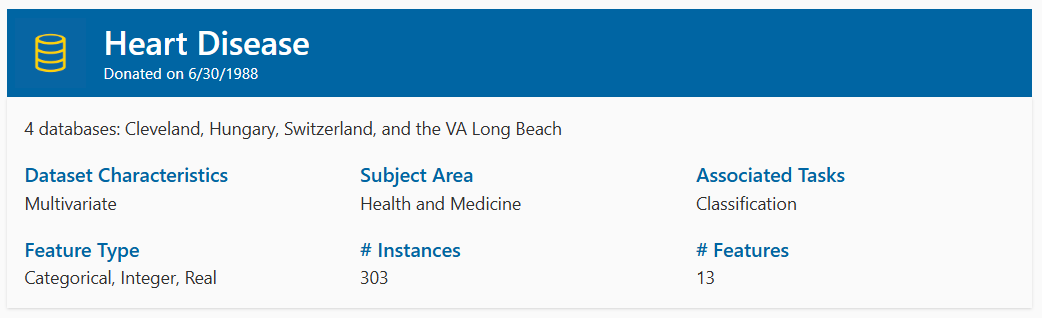
\includegraphics[width=0.485\textwidth]{imagens/dataset titulo.png}
    \caption{Página inicial Base de dados}
    \label{capa}
\end{figure}
A base de dados utilizada neste estudo foi obtida a partir do repositório da UCI Machine Learning Repository \cite{Dataset}. Embora originalmente a base contenha um número maior de parâmetros, nesta análise optou-se por utilizar um conjunto específico de variáveis que se demonstraram relevantes tanto para a predição de doenças cardíacas quanto para a interpretação clínica dos resultados. Os parâmetros selecionados foram:

\begin{itemize}
    \item \textbf{age} (idade): Refere-se à idade do paciente. A idade é um fator de risco fundamental para doenças cardiovasculares, uma vez que o envelhecimento está associado a alterações fisiológicas que podem predispor a problemas cardíacos.
    \item \textbf{sex} (sexo): Indica o gênero do paciente, codificado como 0 para feminino e 1 para masculino. Estudos epidemiológicos sugerem que a incidência e a manifestação das doenças cardíacas podem variar entre os sexos, tornando este parâmetro crucial para a análise comparativa e estratificação do risco.
    \item \textbf{chestPain} (tipo de dor no peito): Representa a natureza da dor torácica experimentada pelo paciente, podendo indicar diferentes tipos de angina ou outras condições. A caracterização da dor no peito é importante, pois permite inferir a possível presença de isquemia ou outros problemas coronarianos.
    \item \textbf{restingBloodPressure} (pressão arterial em repouso): Mede a pressão arterial do paciente enquanto este está em repouso. Pressões elevadas estão frequentemente associadas a um maior risco de eventos cardíacos e podem ser um indicativo de hipertensão, um dos principais fatores de risco para doenças do coração.
    \item \textbf{serumCholestoral} (colesterol sérico): Indica o nível de colesterol presente no sangue. Altos níveis de colesterol podem contribuir para o desenvolvimento de placas ateroscleróticas, aumentando significativamente o risco de infarto e outras complicações cardiovasculares.
    \item \textbf{restingEletroc} (resultados do eletrocardiograma em repouso): Fornece informações sobre a atividade elétrica do coração enquanto o paciente está em repouso. Anomalias neste exame podem sugerir a presença de arritmias ou outras disfunções que estão associadas a uma maior propensão a eventos cardíacos.
    \item \textbf{maximumHeartRate} (frequência cardíaca máxima): Representa a frequência cardíaca máxima atingida pelo paciente durante um teste de esforço. Este parâmetro é relevante para avaliar a resposta do coração ao exercício e pode indicar a capacidade funcional do sistema cardiovascular, bem como a presença de possíveis limitações.
    \item \textbf{exerciseInducedAngina} (angina induzida pelo exercício): Indica se o paciente apresenta dor no peito durante o esforço físico. A presença de angina induzida pelo exercício é um sinal importante de que o coração pode estar sofrendo de isquemia, evidenciando uma resposta inadequada ao aumento da demanda metabólica.
    \item \textbf{diagnosis} (diagnóstico): Variável alvo que indica a presença ou ausência de doença cardíaca. Este parâmetro é utilizado para treinar e validar o classificador, permitindo a comparação dos resultados preditivos com o diagnóstico clínico real.
\end{itemize}
Cada um desses parâmetros foi escolhido por sua relevância clínica e potencial para influenciar a predição de doenças cardíacas. A combinação destes atributos permite não apenas a construção de um modelo preditivo robusto, mas também a realização de uma análise aprofundada sobre os fatores de risco e as características dos pacientes, contribuindo para uma abordagem integrada que une técnicas de aprendizado de máquina e conhecimento médico.

\section{Análise Exploratória dos dados}
Nesta seção, descrevemos as principais análises exploratórias realizadas a partir do código desenvolvido, o qual gerou diversos gráficos para investigar as relações entre os parâmetros do dataset e o diagnóstico de doenças cardíacas.

\subsection{Visualizações para Variáveis Contínuas}
Foram gerados gráficos de dispersão (scatter plots) relacionando as variáveis contínuas com o diagnóstico, possibilitando a observação das distribuições e tendências:
\begin{itemize}
    \begin{figure}[htbp]
        \centering
        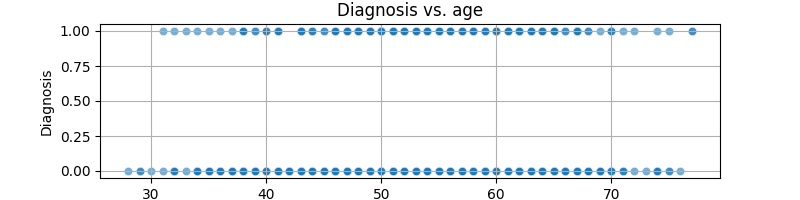
\includegraphics[width=0.485\textwidth]{imagens/age.png}
        \caption{Distribuição de idades dos pacientes}
        \label{idade}
    \end{figure}
    \item \textbf{Diagnosis vs. Age:} O gráfico demonstra que a distribuição da variável \textit{age} (idade) está bem espalhada entre os casos positivos (diagnóstico 1) e negativos (diagnóstico 0), indicando que, embora a idade seja um fator de risco, ela não se mostra isoladamente determinante para a presença da doença.
    
    \begin{figure}[htbp]
        \centering
        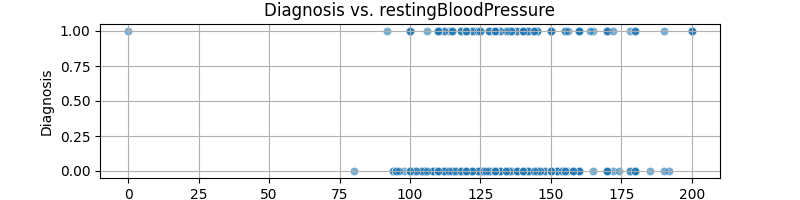
\includegraphics[width=0.485\textwidth]{imagens/restingBloodPressure.png}
        \caption{Pressão arterial em repouso}
        \label{pressao_repouso}
    \end{figure}
    \item \textbf{Diagnosis vs. Resting Blood Pressure:} Observa-se que os valores para pacientes com diagnóstico 0 se distribuem amplamente na faixa de aproximadamente 85 a 190 mmHg, enquanto os pacientes com diagnóstico 1 apresentam uma concentração maior dos valores entre 110 e 145 mmHg. Essa diferença sugere que, para esta amostra, pressões mais moderadas podem estar associadas à manifestação da doença.
    
    \begin{figure}[htbp]
        \centering
        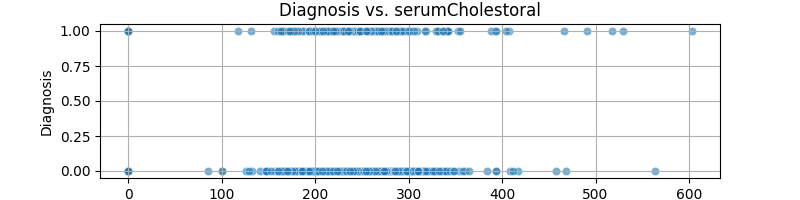
\includegraphics[width=0.485\textwidth]{imagens/serumCholestoral.png}
        \caption{Níveis séricos de colesterol}
        \label{colesterol}
    \end{figure}
    \item \textbf{Diagnosis vs. Serum Cholestoral:} A análise do colesterol sérico mostrou uma distribuição homogênea entre os grupos, sem evidenciar uma concentração específica para nenhum dos diagnósticos, o que pode indicar que, quando analisado isoladamente, este parâmetro não diferencia de forma clara os pacientes doentes dos saudáveis.
    
    \begin{figure}[htbp]
        \centering
        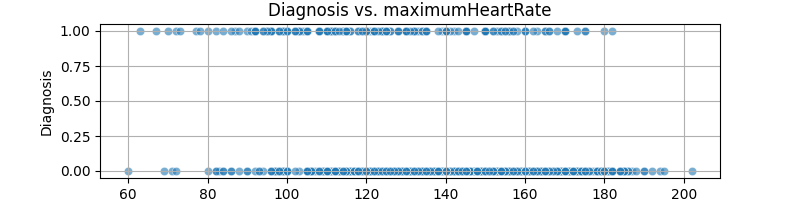
\includegraphics[width=0.485\textwidth]{imagens/maximumHeartRate.png}
        \caption{Frequência cardíaca máxima observada}
        \label{freq_card_max}
    \end{figure}
    \item \textbf{Diagnosis vs. Maximum Heart Rate:} O gráfico evidencia que a frequência cardíaca máxima dos pacientes durante testes de esforço também apresenta uma distribuição semelhante entre os grupos, sugerindo que outros fatores associados ao teste de esforço podem contribuir para a diferenciação diagnóstica.
\end{itemize}

\subsection{Visualizações para Variáveis Discretas}
Para as variáveis discretas, foram gerados gráficos de barras que permitem a contagem dos casos de diagnóstico para cada categoria:
\begin{itemize}
    \begin{figure}[htbp]
        \centering
        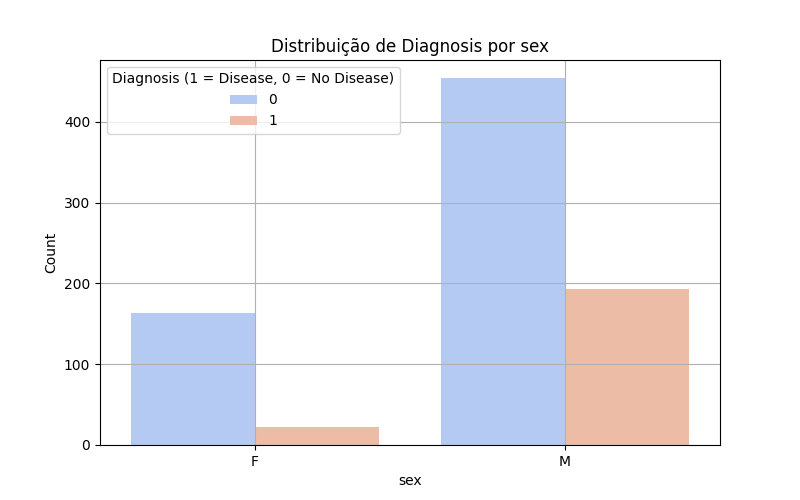
\includegraphics[width=0.485\textwidth]{imagens/sex.png}
        \caption{Distribuição por sexo dos pacientes}
        \label{sexo}
    \end{figure}
    \item \textbf{Diagnosis por Sex:} A distribuição dos diagnósticos por sexo evidencia a predominância de homens na base de dados, tanto no total quanto no número de casos positivos. Além disso, a proporção de homens com diagnóstico 1 é significativamente maior quando comparada à proporção observada em mulheres.
    
    \begin{figure}[htbp]
        \centering
        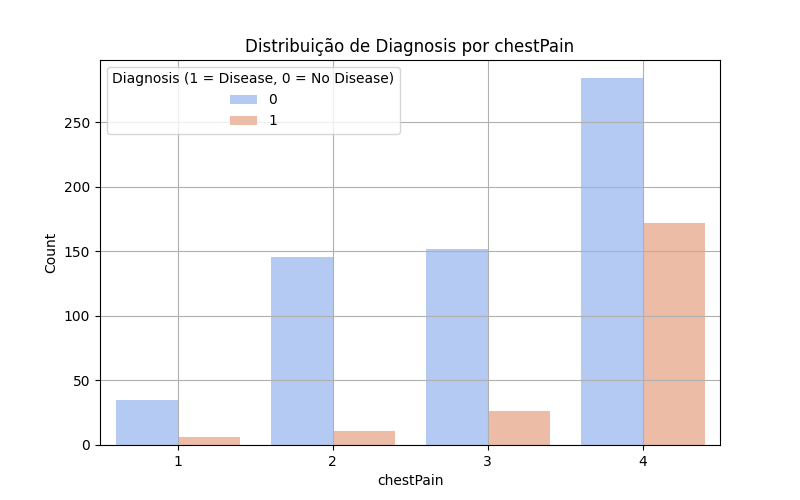
\includegraphics[width=0.485\textwidth]{imagens/chestPain.png}
        \caption{Tipos de dor torácica relatados}
        \label{dor_torax}
    \end{figure}
    \item \textbf{Diagnosis por ChestPain:} Os gráficos demonstram que, conforme o tipo ou intensidade da dor no peito aumenta (representado por maiores valores da variável \textit{chestPain}), há um aumento no número de diagnósticos positivos. Esse resultado reforça a relevância clínica da característica da dor torácica para a avaliação do risco cardiovascular.
    

    \begin{figure}[htbp]
        \centering
        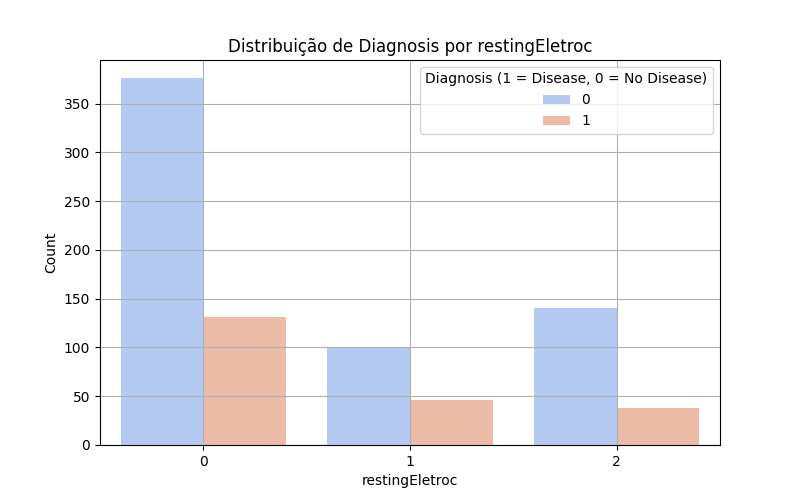
\includegraphics[width=0.485\textwidth]{imagens/restingEletroc.png}
        \caption{Resultados eletrocardiográficos em repouso}
        \label{eletro_repouso}
    \end{figure}
    \item \textbf{Diagnosis por Resting Eletroc:} A análise dos resultados do eletrocardiograma em repouso mostra uma distribuição que contribui para a compreensão de anomalias elétricas associadas a diferentes diagnósticos, embora não haja uma tendência tão marcante quanto em outros parâmetros.
    
    \begin{figure}[htbp]
        \centering
        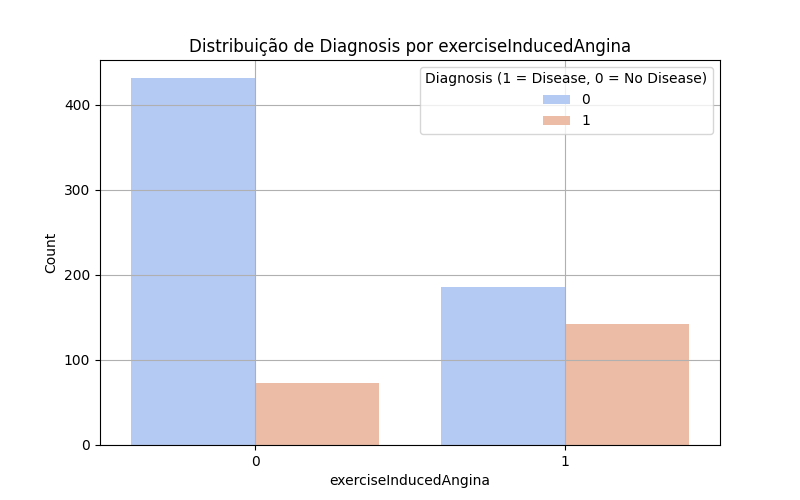
\includegraphics[width=0.485\textwidth]{imagens/exerciseInducedAngina.png}
        \caption{Presença de angina induzida por exercício}
        \label{angina}
    \end{figure}
    \item \textbf{Diagnosis por ExerciseInducedAngina:} Observa-se que a incidência de diagnósticos positivos aumenta consideravelmente quando \textit{exerciseInducedAngina} assume o valor 1. Esse resultado é coerente com a hipótese de que a presença de angina induzida pelo exercício é um forte indicador de isquemia e, consequentemente, de doença cardíaca.
\end{itemize}

\subsection{Análise de Correlação}
Além das visualizações individuais, foi gerado um heatmap que ilustra a correlação entre cada parâmetro e o diagnóstico. A partir desse mapa de calor, pode-se observar:
\begin{itemize}
    \begin{figure}[htbp]
        \centering
        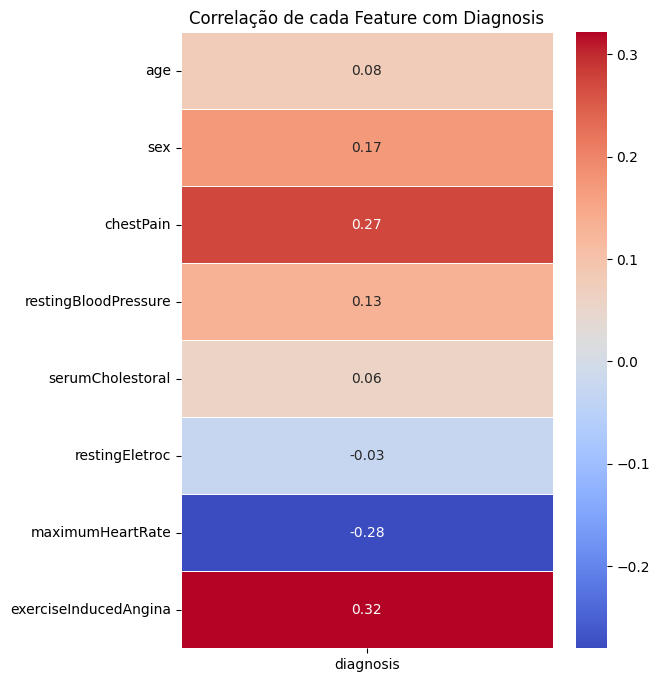
\includegraphics[width=0.4\textwidth]{imagens/heatmap.png}
        \caption{Heatmap de correlação entre variáveis}
        \label{heatmap}
    \end{figure}    
    \item \textbf{Contribuição Positiva para Diagnóstico 1:} Valores elevados nas variáveis \textit{chestPain} e \textit{exerciseInducedAngina} estão fortemente associados a diagnósticos positivos, indicando que a presença e intensidade da dor no peito, assim como a ocorrência de angina durante exercícios, são indicadores importantes da presença de doenças cardíacas.
    \item \textbf{Contribuição para Diagnóstico 0:} Por outro lado, valores elevados em \textit{maximumHeartRate} e \textit{restingEletroc} tendem a estar correlacionados com diagnósticos negativos, sugerindo que melhores respostas ao esforço e padrões eletrocardiográficos mais regulares podem indicar um menor risco de doença.
\end{itemize}

\subsection{Medidas de Dispersão}
Adicionalmente, foram computadas diversas medidas de dispersão para cada parâmetro, como mínimo, máximo, amplitude, média, mediana, variância, desvio padrão, coeficiente de variação e quartis. Essas estatísticas permitem uma visão detalhada da distribuição dos dados, fornecendo subsídios para a compreensão dos comportamentos individuais das variáveis e a identificação de possíveis outliers ou assimetrias que possam influenciar a análise preditiva.

Em suma, a análise exploratória dos dados revelou informações importantes sobre a distribuição dos parâmetros e suas relações com o diagnóstico de doenças cardíacas. Tais insights são fundamentais para embasar a construção do modelo preditivo, bem como para a interpretação dos resultados obtidos no contexto clínico.


\section{Classificador Ingênuo de Bayes}
O classificador ingênuo de Bayes é uma técnica de aprendizado de máquina baseada no teorema de Bayes, que utiliza uma abordagem probabilística para a classificação. Apesar da suposição simplificadora de independência condicional entre os atributos, essa metodologia tem se mostrado eficiente em diversas aplicações, inclusive na área da saúde para a predição de doenças cardíacas.

\subsection{Fundamentos Teóricos}
O teorema de Bayes estabelece uma relação entre a probabilidade condicional de um evento e a sua probabilidade inversa. Matematicamente, para um conjunto de classes $C = \{C_1, C_2, \ldots, C_k\}$ e um vetor de atributos $x = (x_1, x_2, \ldots, x_n)$, o teorema é expresso como:
\[
P(C_k \mid x) = \frac{P(x \mid C_k) \, P(C_k)}{P(x)}
\]
onde:
\begin{itemize}
    \item $P(C_k \mid x)$ é a probabilidade a posteriori de que o vetor de atributos $x$ pertença à classe $C_k$;
    \item $P(x \mid C_k)$ é a verossimilhança, ou seja, a probabilidade de observar o vetor $x$ dado que a classe é $C_k$;
    \item $P(C_k)$ é a probabilidade a priori da classe $C_k$;
    \item $P(x)$ é a probabilidade de observar o vetor $x$, atuando como uma constante de normalização.
\end{itemize}

Na prática, como $P(x)$ é constante para todas as classes, o classificador ingênuo de Bayes opta por calcular a probabilidade proporcional:
\[
P(C_k \mid x) \propto P(x \mid C_k) \, P(C_k)
\]
e a decisão de classificação é feita selecionando a classe que maximiza essa probabilidade, ou seja:
\[
\hat{C} = \arg \max_{C_k \in C} \; P(x \mid C_k) \, P(C_k)
\]

\subsection{Assunção de Independência Condicional}
A principal suposição que torna o classificador \textit{ingênuo} é a hipótese de que os atributos são condicionalmente independentes, dado a classe. Formalmente, isso pode ser escrito como:
\[
P(x \mid C_k) = \prod_{i=1}^{n} P(x_i \mid C_k)
\]
Essa simplificação permite que o cálculo da verossimilhança seja realizado de maneira eficiente, uma vez que a estimativa conjunta de $P(x \mid C_k)$ é decomposta em produtos de probabilidades individuais para cada atributo. Apesar de, na prática, os atributos frequentemente apresentarem alguma correlação, essa aproximação tem se mostrado eficaz em muitos problemas reais.

\subsection{Modelagem das Probabilidades}
A implementação prática do classificador ingênuo de Bayes requer a estimativa das seguintes probabilidades:
\begin{enumerate}
    \item \textbf{Probabilidade a Priori $P(C_k)$:} É calculada a partir da frequência de cada classe no conjunto de treinamento. Se $N$ é o número total de amostras e $N_k$ é o número de amostras pertencentes à classe $C_k$, então:
    \[
    P(C_k) = \frac{N_k}{N}
    \]
    \item \textbf{Verossimilhança $P(x_i \mid C_k)$:} A forma dessa probabilidade depende do tipo de atributo:
    \begin{itemize}
        \item Para atributos discretos, pode-se utilizar a frequência relativa de ocorrência de cada valor em uma dada classe;
        \item Para atributos contínuos, é comum assumir que os dados seguem uma distribuição normal (gaussiana). Nesse caso, a verossimilhança é dada por:
        \[
        P(x_i \mid C_k) = \frac{1}{\sqrt{2\pi\sigma_{ik}^2}} \exp\left( -\frac{(x_i - \mu_{ik})^2}{2\sigma_{ik}^2} \right)
        \]
        onde $\mu_{ik}$ e $\sigma_{ik}$ são, respectivamente, a média e o desvio padrão do atributo $x_i$ para a classe $C_k$.
    \end{itemize}
\end{enumerate}

\subsection{Decisão e Classificação}
Após a estimativa das probabilidades a priori e das verossimilhanças para cada atributo, o classificador calcula a probabilidade a posteriori para cada classe e realiza a decisão de classificação utilizando o critério de máxima verossimilhança (MAP):
\[
\hat{C} = \arg \max_{C_k \in C} \; \left( P(C_k) \prod_{i=1}^{n} P(x_i \mid C_k) \right)
\]
Esse método é computacionalmente eficiente e, apesar da suposição de independência que pode ser considerada exagerada em alguns contextos, ele frequentemente produz resultados robustos e interpretáveis.

\subsection{Vantagens e Limitações}
Entre as principais vantagens do classificador ingênuo de Bayes, destacam-se:
\begin{itemize}
    \item \textbf{Simplicidade e Eficiência:} A decomposição do cálculo das probabilidades em termos individuais reduz a complexidade computacional, permitindo a aplicação em grandes conjuntos de dados.
    \item \textbf{Baixa Dimensionalidade:} A independência condicional facilita a interpretação dos impactos de cada variável.
    \item \textbf{Aplicabilidade em Diversos Domínios:} Apesar da suposição simplificada, o modelo é amplamente utilizado em áreas como filtragem de spam, análise de sentimentos e, como demonstrado neste estudo, na predição de doenças cardíacas.
\end{itemize}

Entretanto, a principal limitação reside na suposição de independência entre os atributos. Em cenários onde os atributos são fortemente correlacionados, essa aproximação pode afetar a precisão do modelo. Técnicas de suavização, como a suavização de Laplace, podem ser aplicadas para mitigar problemas decorrentes de probabilidades zero em dados esparsos, garantindo uma estimativa mais robusta.

Em resumo, o classificador ingênuo de Bayes oferece um equilíbrio entre simplicidade e desempenho, servindo como uma ferramenta valiosa para a análise preditiva e a interpretação dos dados, especialmente em contextos onde a transparência e a eficiência são fundamentais.

\section{Experimentos}
Para validar o desempenho do classificador ingênuo de Bayes, foram adotadas diversas estratégias de teste e avaliação, visando garantir a robustez dos resultados e a capacidade de generalização do modelo. Cada método implementado permite explorar diferentes aspectos do comportamento do classificador, proporcionando uma análise abrangente de sua eficácia. A seguir, são descritas as abordagens utilizadas:

\subsection{Hold-Out}
A abordagem de Hold-Out consiste em dividir o conjunto de dados em duas partes distintas: um conjunto de treinamento e um conjunto de teste. Nesta estratégia, uma parcela dos dados (geralmente entre 70\% e 80\%) é utilizada para treinar o modelo, enquanto o restante serve para avaliar sua performance. Essa divisão permite uma avaliação rápida e prática do desempenho preditivo, fornecendo métricas como acurácia, precisão, sensibilidade e F1-score. Apesar de sua simplicidade, o método Hold-Out pode sofrer com a variabilidade dos resultados, dependendo da forma como os dados são particionados.

\subsection{Bootstrap}
A técnica de Bootstrap é uma abordagem de reamostragem que gera múltiplos conjuntos de dados a partir do dataset original, por meio de amostragem com reposição. Cada conjunto reamostrado é utilizado para treinar e testar o modelo, possibilitando a estimativa da variabilidade das métricas de desempenho e a construção de intervalos de confiança para os resultados. Essa metodologia é particularmente útil quando se deseja obter uma visão mais robusta da estabilidade do classificador, mesmo em cenários com conjuntos de dados limitados.

\subsection{Cross Validation}
A validação cruzada (Cross Validation) é uma técnica amplamente utilizada para avaliar a performance dos modelos de forma mais estável e menos dependente de uma única divisão dos dados. No contexto deste projeto, foi empregado o método de K-Fold, onde o conjunto de dados é dividido em $K$ partes iguais. Em cada iteração, o modelo é treinado utilizando $K-1$ folds e testado no fold restante. A média dos resultados obtidos em todas as iterações fornece uma estimativa mais confiável do desempenho do classificador.

\subsection{Stratified K-Fold}
Uma variação da validação cruzada, o Stratified K-Fold, foi também aplicada para garantir que cada partição dos dados mantenha a mesma proporção de classes presente no dataset original. Essa estratificação é especialmente relevante em problemas de classificação onde as classes podem estar desbalanceadas, como no caso da predição de doenças cardíacas. Ao assegurar que cada fold reflita a distribuição original, é possível obter uma avaliação mais realista e menos tendenciosa do desempenho do modelo.

\subsection{Integração dos Resultados}
Cada uma das abordagens descritas foi implementada em notebooks específicos (Bootstrap, Cross Validation e Stratified K-Fold) e, juntamente com os resultados obtidos através do método Hold-Out, permitiu uma análise detalhada dos seguintes aspectos:
\begin{itemize}
    \item \textbf{Robustez e Generalização:} Através do uso de reamostragem (Bootstrap) e de validação cruzada, foi possível avaliar como o modelo se comporta em diferentes subconjuntos dos dados, minimizando o risco de overfitting e proporcionando uma estimativa mais confiável do desempenho em dados não vistos.
    \item \textbf{Variabilidade dos Resultados:} O emprego de múltiplas abordagens evidenciou a variabilidade inerente ao processo de treinamento e teste, possibilitando a construção de intervalos de confiança para as métricas e a identificação de possíveis fontes de instabilidade.
    \item \textbf{Distribuição das Classes:} O uso do Stratified K-Fold, em particular, assegurou que a avaliação fosse realizada de forma justa, preservando a proporção original das classes, o que é crucial em cenários com classes desbalanceadas, como a detecção de doenças cardíacas.
\end{itemize}

Em resumo, a fase de teste e avaliação combinou métodos tradicionais e avançados para oferecer uma visão completa do desempenho do classificador ingênuo de Bayes. Essa abordagem múltipla permitiu validar a eficácia do modelo sob diferentes perspectivas, contribuindo para uma análise mais confiável e fundamentada no contexto clínico e preditivo.

\section{Análise dos resultados}
A partir da aplicação do classificador ingênuo de Bayes utilizando diferentes estratégias de validação (Hold-Out, Bootstrap, Cross Validation e Stratified K-Fold), foi possível obter uma visão abrangente do desempenho do modelo e identificar aspectos relevantes sobre sua robustez e consistência.

\subsection{Consistência entre os Métodos de Validação}
Observou-se que os resultados se mantiveram relativamente consistentes entre os diferentes métodos de avaliação. Em particular:
\begin{itemize}
    \item \textbf{Hold-Out:} A divisão inicial dos dados em treinamento e teste permitiu uma avaliação rápida, evidenciando um desempenho promissor do modelo em termos de acurácia, precisão e sensibilidade. Entretanto, a variação inerente a uma única divisão pode não refletir completamente a capacidade de generalização.
    \begin{figure}[htbp]
        \centering
        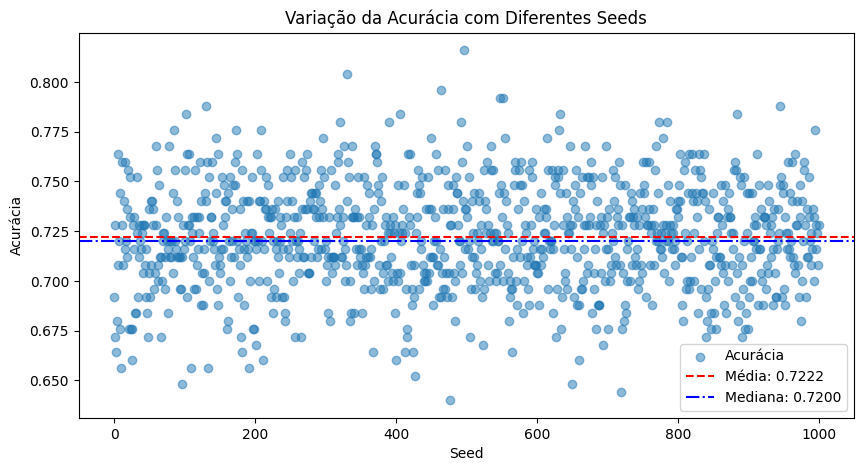
\includegraphics[width=0.485\textwidth]{imagens/Hold-Out.png}
        \caption{Variação da acurácia pelo método Hold-Out}
        \label{hold_out}
    \end{figure}
    
    \item \textbf{Bootstrap:} A técnica de reamostragem evidenciou a estabilidade das métricas ao longo de múltiplas amostragens do conjunto original. A construção de intervalos de confiança para as métricas de desempenho reforçou a robustez do classificador, minimizando os efeitos de variações pontuais na amostragem.
    \begin{figure}[htbp]
        \centering
        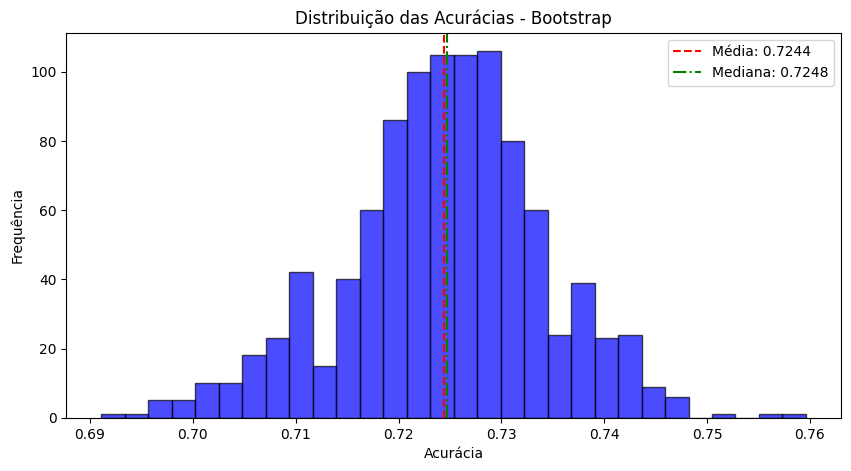
\includegraphics[width=0.485\textwidth]{imagens/bootstrap1.png}
        \caption{Bootstrap - Distribuição das acurácias}
        \label{bootstrap_amostras}
    \end{figure}
    \begin{figure}[htbp]
        \centering
        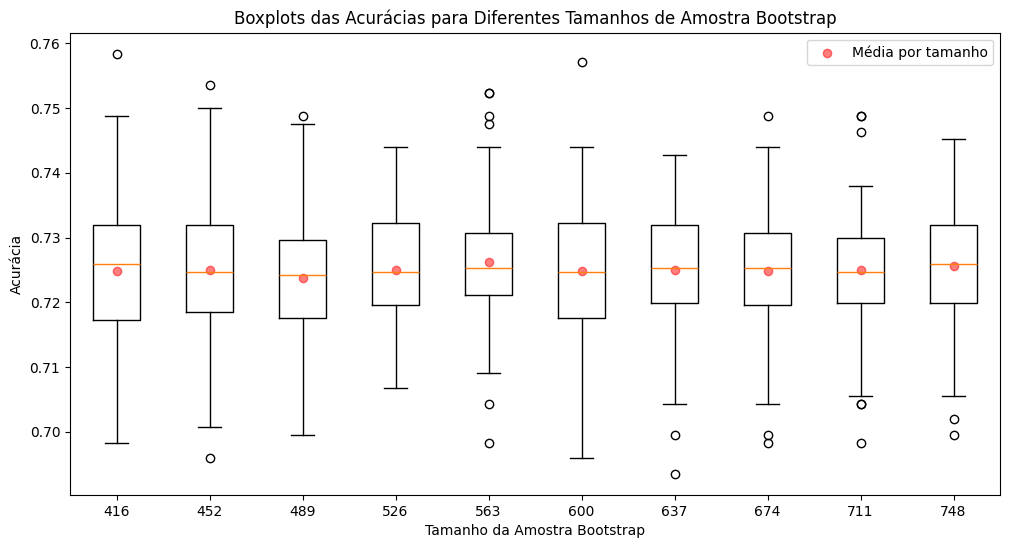
\includegraphics[width=0.485\textwidth]{imagens/bootstrap2.png}
        \caption{Bootstrap - Box plot}
        \label{bootstrap_distribuicao}
    \end{figure}
    
    \item \textbf{Cross Validation e Stratified K-Fold:} Essas abordagens permitiram uma avaliação mais detalhada e imparcial do modelo, especialmente em cenários onde a distribuição das classes apresenta desbalanceamento. A preservação das proporções originais das classes no Stratified K-Fold foi fundamental para uma análise justa e mostrou que o desempenho do classificador permanece estável mesmo quando os dados são particionados de formas distintas.
    \begin{figure}[htbp]
        \centering
        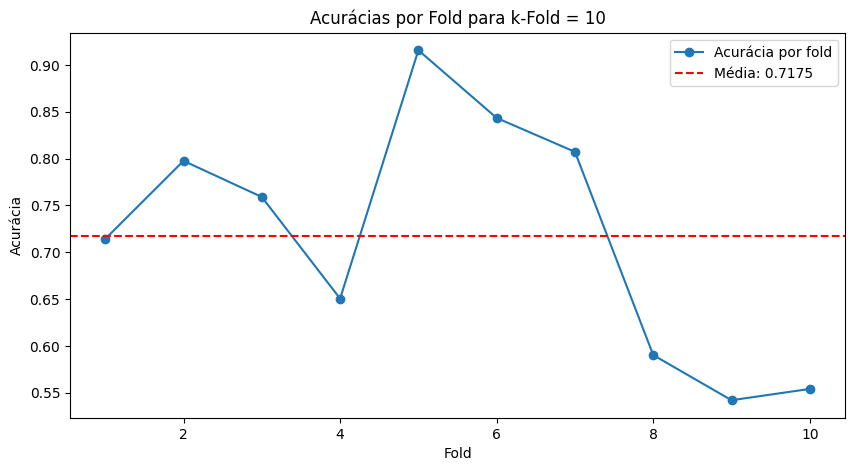
\includegraphics[width=0.485\textwidth]{imagens/crossValidation1.png}
        \caption{Acurácias por numero de folds}
        \label{cross_val_etapas}
    \end{figure}
    \begin{figure}[htbp]
        \centering
        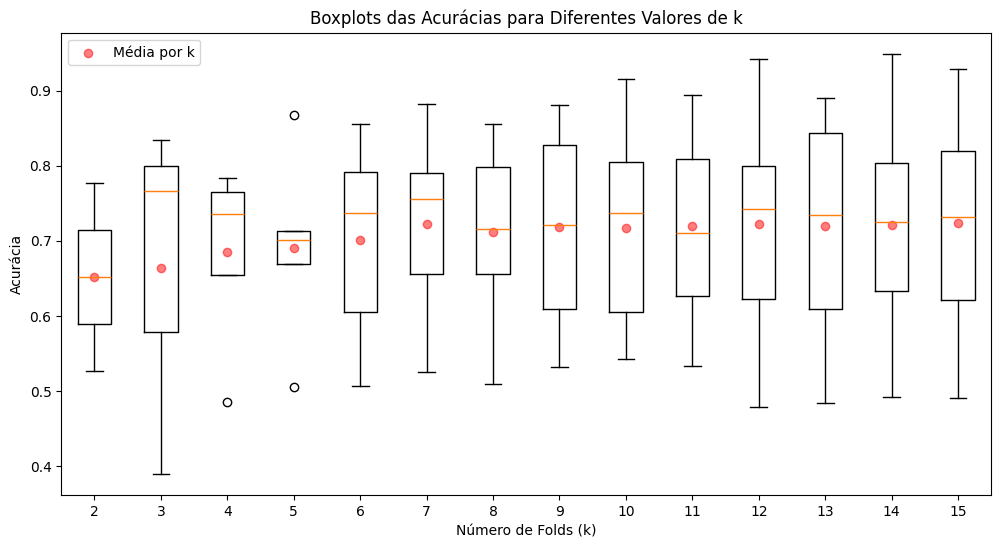
\includegraphics[width=0.485\textwidth]{imagens/crossValidation2.png}
        \caption{Validação cruzada K-Fold - Box blot}
        \label{cross_val_resultados}
    \end{figure}
\end{itemize}

\subsection{Interpretação dos Resultados no Contexto Clínico}
A análise dos resultados também trouxe insights importantes para a aplicação prática no contexto da saúde:
\begin{itemize}
    \item A consistência dos resultados entre os diferentes métodos de validação sugere que o modelo possui boa capacidade de generalização para novos dados, o que é crucial para sua aplicação em ambientes clínicos.
    \item Os parâmetros que apresentaram forte correlação com o diagnóstico, como \textit{chestPain} e \textit{exerciseInducedAngina}, corroboram a relevância clínica desses indicadores na avaliação do risco cardiovascular.
    \item Por outro lado, a identificação de que parâmetros como \textit{maximumHeartRate} e \textit{restingEletroc} estão mais associados a diagnósticos negativos pode oferecer subsídios para uma análise diferenciada e para a definição de estratégias de intervenção precoce.
\end{itemize}

\section{Conclusões e discussões}
Em síntese, a análise dos resultados demonstra que o classificador ingênuo de Bayes, mesmo com a sua simplificação teórica, se mostra uma ferramenta eficaz para a predição de doenças cardíacas quando aplicado ao conjunto de dados selecionado. A utilização de múltiplas abordagens de validação, como o Hold-Out, Bootstrap, Cross Validation e Stratified K-Fold, reforça a confiabilidade dos resultados, sugerindo que, apesar das limitações inerentes à hipótese de independência, o modelo apresenta desempenho robusto e potencial aplicabilidade em contextos de saúde preventiva.

Do ponto de vista metodológico, a simplicidade do classificador ingênuo de Bayes se revelou vantajosa, permitindo uma implementação rápida e uma interpretação transparente dos resultados. A decomposição do problema em probabilidades individuais facilitou a análise dos fatores de risco e a compreensão dos indicadores clínicos, como \textit{chestPain} e \textit{exerciseInducedAngina}, que se mostraram fortemente correlacionados com a presença da doença. Essa abordagem não só viabiliza a tomada de decisão em tempo hábil, mas também contribui para a elaboração de estratégias de intervenção e prevenção.

Contudo, é importante ressaltar que a suposição de independência entre os atributos, embora prática, pode não refletir a complexidade real das interações entre os diversos fatores de risco. Essa limitação sugere que, em aplicações futuras, a combinação do classificador ingênuo de Bayes com outras técnicas ou a inclusão de métodos que consigam capturar a correlação entre variáveis pode levar a uma melhoria ainda maior na acurácia preditiva e na identificação dos casos críticos.

Além disso, a análise das métricas de desempenho e a consistência dos resultados obtidos através das diversas técnicas de validação indicam uma boa capacidade de generalização do modelo, o que é um aspecto crucial para a sua aplicação em ambientes clínicos. A integração dos resultados das diferentes metodologias de avaliação também possibilitou a identificação de potenciais fontes de instabilidade e a construção de intervalos de confiança, fornecendo subsídios para um embasamento estatístico mais robusto.

Por fim, a experiência obtida neste estudo contribui para a discussão sobre a aplicação de técnicas de aprendizado de máquina na área da saúde, especialmente no que diz respeito à predição e prevenção de doenças cardiovasculares. A viabilidade do classificador ingênuo de Bayes, aliada à interpretação dos indicadores clínicos, demonstra o potencial dessas abordagens para auxiliar profissionais da saúde na identificação precoce de pacientes em risco, promovendo intervenções mais assertivas e a implementação de políticas de saúde pública mais direcionadas.

Em termos de trabalhos futuros, recomenda-se explorar a integração de modelos híbridos, bem como o uso de técnicas de seleção de atributos e de engenharia de características, a fim de mitigar as limitações da hipótese de independência e aprimorar a capacidade preditiva do modelo. Dessa forma, este estudo não só reafirma a utilidade do classificador ingênuo de Bayes no contexto de doenças cardíacas, como também aponta caminhos promissores para o avanço das ferramentas de análise preditiva na área da saúde.

\begin{thebibliography}{00}
    \bibitem{Dataset} A. Janosi, W. Steinbrunn, M. Pfisterer, and R. Detrano, ``Heart Disease Data Set,'' \textit{UCI Machine Learning Repository}, 1988. [Online]. Disponível em: \url{https://archive.ics.uci.edu/dataset/45/heart+disease}. Acesso em: 15 mar. 2025.
    \bibitem{Murphy}
    Murphy, K. P. (2012). \textit{Machine Learning: A Probabilistic Perspective}. MIT Press.
    \bibitem{Russell}
    Russell, S. and Norvig, P. (2010). \textit{Artificial Intelligence: A Modern Approach} (3ª ed.). Prentice Hall.
    \bibitem{Hastie}
    Hastie, T., Tibshirani, R. and Friedman, J. (2009). \textit{The Elements of Statistical Learning: Data Mining, Inference, and Prediction} (2ª ed.). Springer.
\end{thebibliography}
\end{document}
